\subsection{水资源治理变化过程}
\label{Res.1}

\begin{figure*}[ht!]
	\centering
	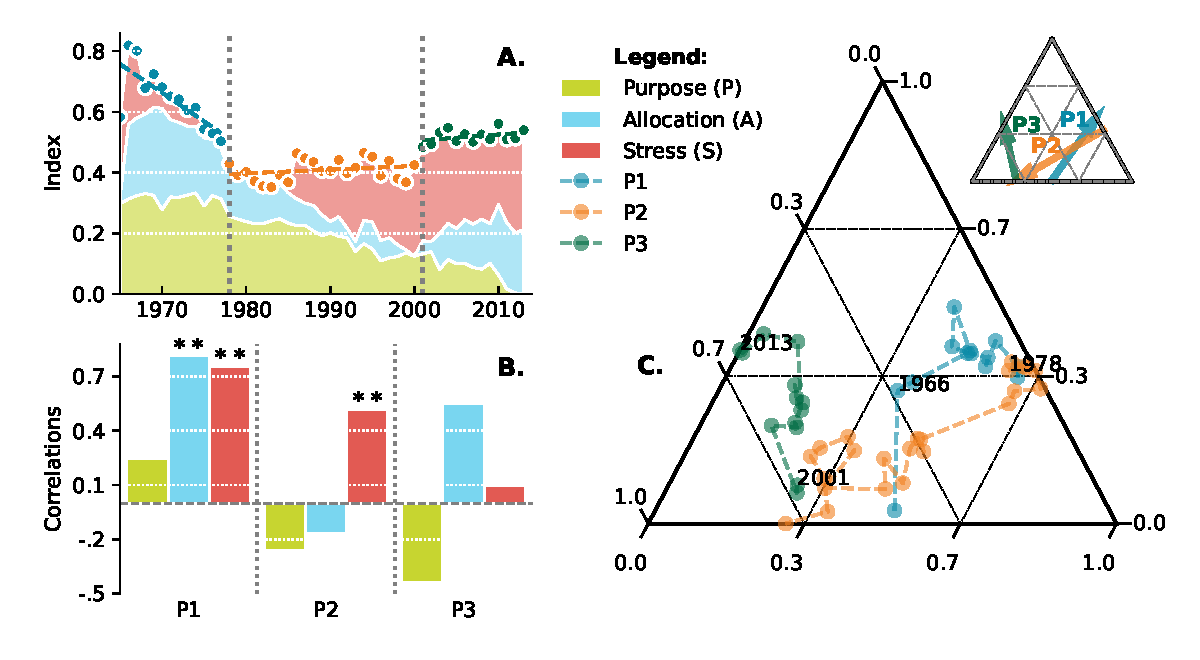
\includegraphics[width=\textwidth]{img/ch4/index.pdf}
	\caption{IWGI指数和相应的水治理制度的变化:P1: 1965-1978, P2: 1979-2001, P3: 2002-2013。
	\textbf{A,} 检测IWGI的变化点和各指标的贡献。1978年和2001年发生了两个重要的变化点($p<0.01$)。
	\textbf{B,}  IWGI与指标之间的趋势相关性。
	\textbf{C,} 在三个指标中,IWGI不断变化的组成部分,其方向在不同的制度之间变化。
	}
	\label{ch4:fig:IWGI}
\end{figure*}

两个重要的断点将IWGI的变化分为三个时期,从三个方面有不同的贡献(图~\ref{ch4:fig:IWGI}A)。
% 第一阶段
IWGI在第一个时期(P1, 1965-1978)迅速下降,虽然目的指标和分配指标对此时期IWGI的贡献更大(平均分别为$49.45\%$和$34.95\%$),但显著的下降趋势($p<0.01$)与分配指标和压力指标的下降显著相关(图~\ref{ch4:fig:IWGI}~B)。
% 第二阶段
在第二阶段(P2, 1979-2001),压力指标的显著增加($p<0.01$)促进了IWGI的上升,而分配指标和目的指标对IWGI的变化起了消极作用。
% 第三阶段

在第三个时期(P3, 1995-2013),虽然压力指标在贡献中保持着最突出的份额(平均为$57.11\%$),但分配指标的增加和目的指标的降低推动了综合指标变化。
%的整体
综上所述,水资源压力、水资源分配、水资源服务三个方面在不同的时期为黄河流域整体特征的变化做出方向性有所差异的贡献(图~\ref{ch4:fig:IWGI}~C)。
